% Tento soubor nahraďte vlastním souborem s přílohami (nadpisy níže jsou pouze pro příklad)

% Pro kompilaci po částech (viz projekt.tex), nutno odkomentovat a upravit
%\documentclass[../projekt.tex]{subfiles}
%\begin{document}

\chapter{RQT Graf hardwarových uzlů}

\begin{figure}[h!]
	\centering
	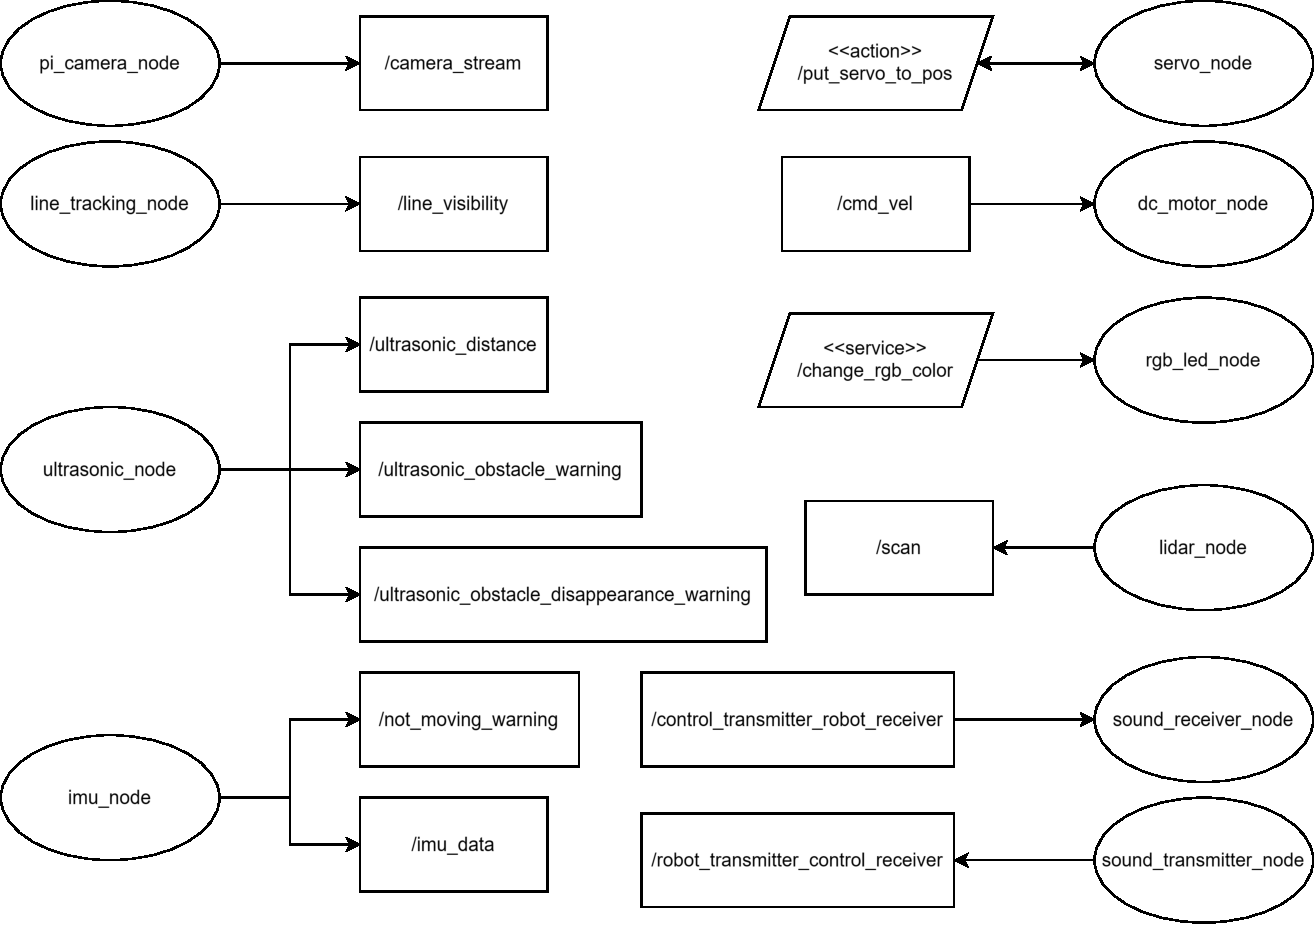
\includegraphics[scale=0.65]{obrazky-figures/hardware_nodes.pdf}
	\caption{RQT Graf hardwarových uzlů a jejich rozhraní}
	\label{}
\end{figure}

\chapter{RQT Graf řídícího systému}

\begin{figure}[h!]
	\centering
	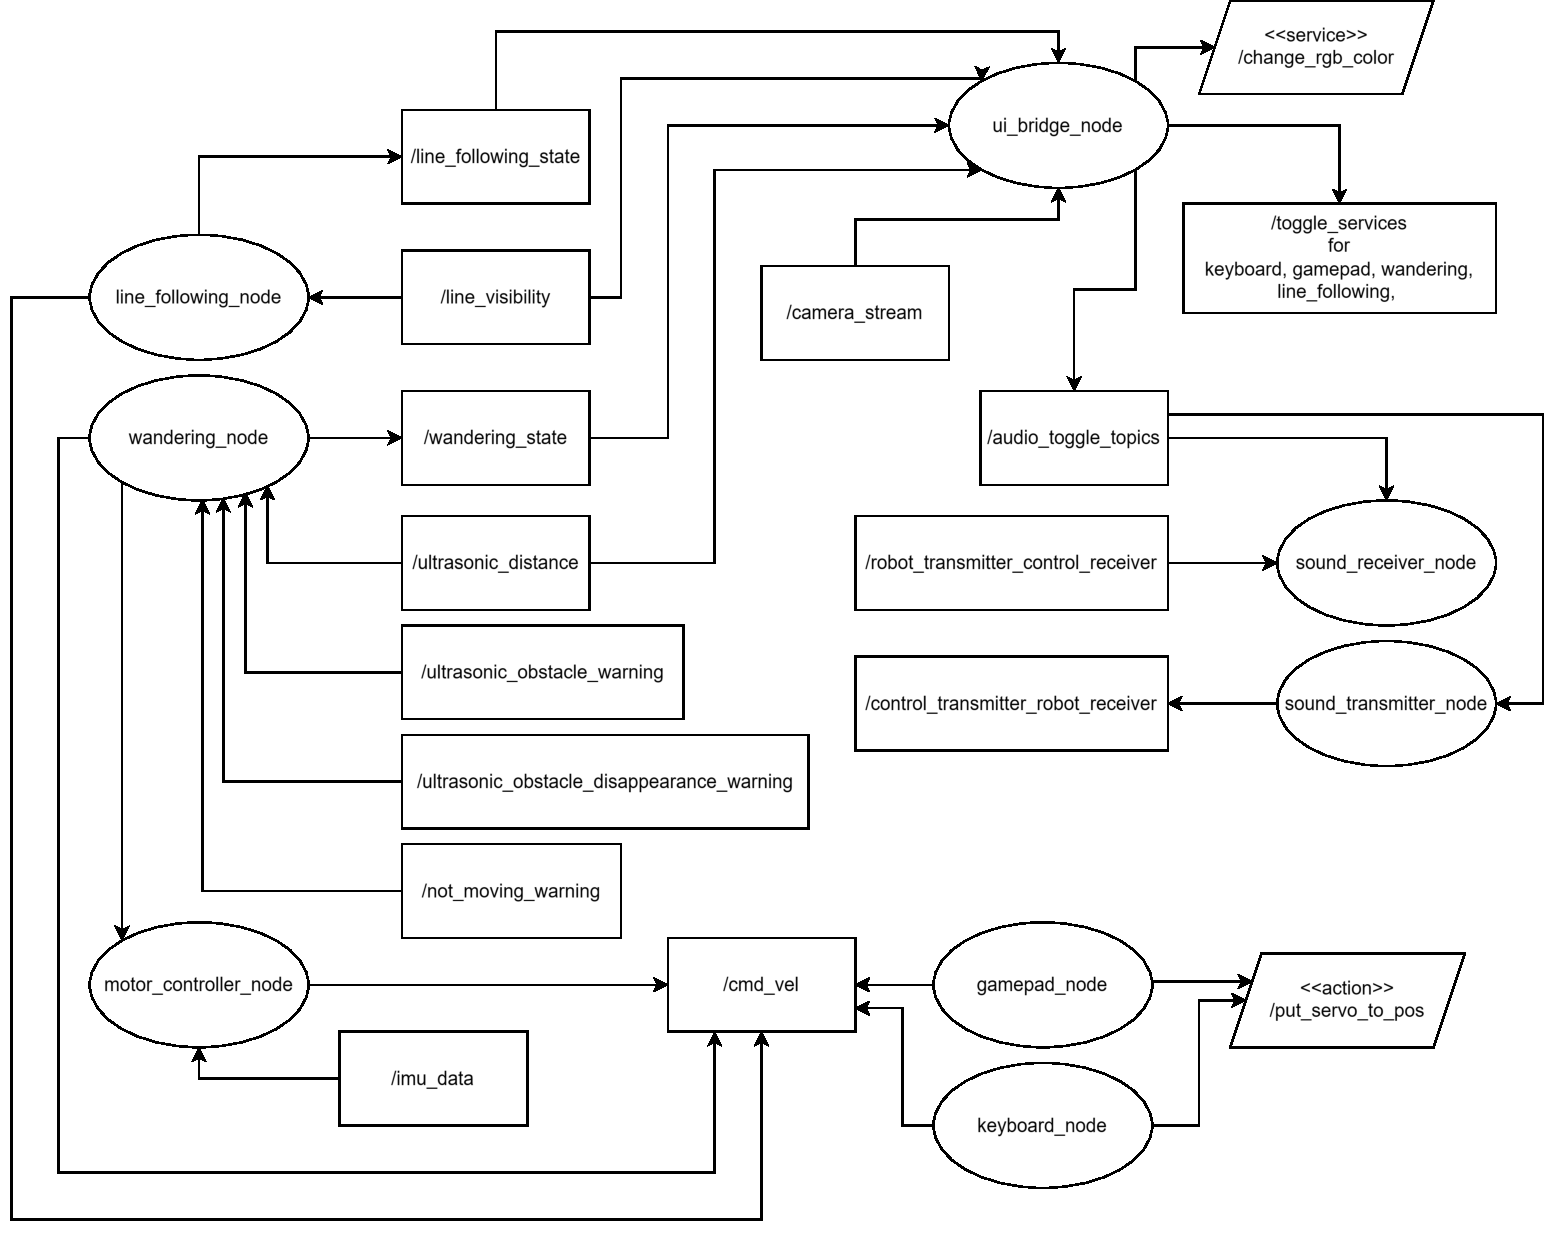
\includegraphics[scale=0.55]{obrazky-figures/controller_nodes.pdf}
	\caption{RQT Graf řídícího systému}
	\label{}
\end{figure}

\chapter{Obsah přiloženého paměťového média}

Struktura paměťového média následuje strukturu ROS2 pracovních ploch. Navíc obsahuje složku \verb|doc| s touto dokumentací. V kořenu se nachází instalační skript a návod na použití.

\begin{center}
	\begin{forest}
		for tree={
			font=\ttfamily,
			grow'=0,
			child anchor=west,
			parent anchor=south,
			anchor=west,
			calign=first,
			inner xsep=7pt,
			edge path={
				\noexpand\path [draw, \forestoption{edge}] (!u.south west) +(7.5pt,0) |- (.child anchor) \forestoption{edge label};
			},
			before typesetting nodes={
				if n=1
				{insert before={[,phantom]}}
				{}
			},
			fit=band,
			before computing xy={l=15pt},
		}
		[Root
		[doc  {\hspace{3em}\# zdrojové latex soubory, tato dokumentace, plakát, video}
		]
		[launch {\hspace{1.5em}\# hromadné spouštěcí soubory}
		]
		[src {\hspace{3em}\# zdrojové soubory vytvořeného systému}
		[adeept\_awr\_diffdrive\_control\_plugin] 
		[adeept\_awr\_nodes]
		[controllers]
		[gazebo\_simulator\_nodes]
		[interfaces]
		]
		[readme.md {\hspace{1.5em}\# návod na použití}]
		[setup.sh  {\hspace{1.5em}\# instalační skript}]
		]
	\end{forest}
\end{center}

% Pro kompilaci po částech (viz projekt.tex) nutno odkomentovat
%\end{document}
